\documentclass[10pt,conference]{IEEEtran}
\usepackage[T1]{fontenc}
\usepackage[utf8]{inputenc}
\usepackage{graphicx}
\usepackage{url}
\usepackage{booktabs}
\usepackage{microtype}

% Working name only: replace this macro when the authors choose a name.
\newcommand{\toolname}{\textsc{ToolName}}
% Visible markers belong to this working draft, not the submission.
\newcommand{\draftnote}[1]{\textit{[#1]}}
\title{From Project Knowledge to Reusable Software Artifacts:\\A Configurable Recommendation Workspace}

% Author order and metadata supplied by the user, converted to IEEEtran.
\author{
\IEEEauthorblockN{Carlos E. M. de Souza\IEEEauthorrefmark{1},
Emanuel Dantas\IEEEauthorrefmark{2},
Ademar Fran\c{c}a de Sousa Neto\IEEEauthorrefmark{3},
Mirko Perkusich\IEEEauthorrefmark{1},\\
Danyllo W. Albuquerque\IEEEauthorrefmark{1},
Kyller Costa Gorg\^onio\IEEEauthorrefmark{1},
Angelo Perkusich\IEEEauthorrefmark{1}}
\IEEEauthorblockA{\IEEEauthorrefmark{1}Federal University of Campina Grande, Campina Grande, Para\'iba, Brazil\\
\IEEEauthorrefmark{2}Federal Institute of Pernambuco, Jaboat\~ao dos Guararapes, Pernambuco, Brazil\\
\IEEEauthorrefmark{3}Federal Rural University of the Semi-Arid Region, Mossor\'o, Rio Grande do Norte, Brazil\\
\{carlos.souza, emanuel.dantas, ademar.sousa\}@virtus.ufcg.edu.br\\
\{danyllo.albuquerque, kyller, perkusich\}@virtus.ufcg.edu.br; mirko@virtus.ufcg.edu.br}
}

\begin{document}
\maketitle
\begin{abstract}
Historical requirements, tests, and project risks are useful only when a team can find relevant artifacts and decide how to reuse them. \toolname{} brings these activities into a web workspace that connects project preparation, taxonomy-guided story classification, configurable recommendation, and human review. Users can publish attributes and reference datasets, run three implemented recommender configurations, inspect the source cases behind a suggestion, and preserve accepted or adapted NFRs and tests. The tool also records the configuration and evidence of each execution, supporting replay after project data change. Our demonstration follows this workflow across non-functional requirements, test cases, and project risks, and shows a configured project feature changing neighbor selection without a dedicated application-code field. A preserved package of 23 technical conditions supports the implemented calculation and compatibility behavior. The demonstration highlights how configurable inputs, visible recommendation origins, and separately recorded decisions make artifact reuse inspectable from preparation to adaptation.
\textbf{Demo video:} \draftnote{YouTube URL pending.}
\end{abstract}
\begin{IEEEkeywords}
software engineering tools, software reuse, recommendation systems, user stories, provenance
\end{IEEEkeywords}

\section{Introduction}
Software projects leave behind requirements, test cases, and knowledge about risks. Reusing an artifact in another context requires more than locating similar text: an engineer needs to understand the context it came from, why it was suggested, and what must change before adoption. User-story taxonomies provide a foundation for linking development assets through functional meaning~\cite{dilorenzo2020wis}. Domain-specific recommenders build on historical information to suggest NFRs~\cite{ramos2025nfr}, tests~\cite{dilorenzo2026testrec}, or project risks~\cite{sousa2026arise}.

\toolname{} turns these reuse activities into a connected workspace. An engineer can prepare a project and its stories, review classifications, choose a recommender, inspect retrieved artifacts and their origins, and record a reuse decision. A researcher or maintainer can configure the attributes and reference data that feed this workflow through the browser. The same application supports story-based recommendation and project-profile recommendation, while retaining the policies specific to each method.

Three capabilities define the demonstration. First, users configure published inputs and dependencies instead of relying on a fixed form for every artifact type. Second, a recommendation remains connected to its source cases, compared features, and execution context. Third, assessments and adapted copies preserve the distinction between retrieved knowledge and the engineer's contribution. Together, these capabilities let the audience follow an artifact from project preparation to an inspectable reuse decision.

\section{The Tool from Preparation to Reuse}
\label{sec:tool}
Figure~\ref{fig:workflow} presents the user journey. The tool offers a project workspace for everyday use and a configuration area for preparing reusable recommenders and reference datasets.

\begin{figure*}[t]
  \centering
  % Vector PDF generated from editable SVG by scripts/build-paper-figures.py
% and scripts/render-paper-figures.ps1. No TikZ dependency is required.
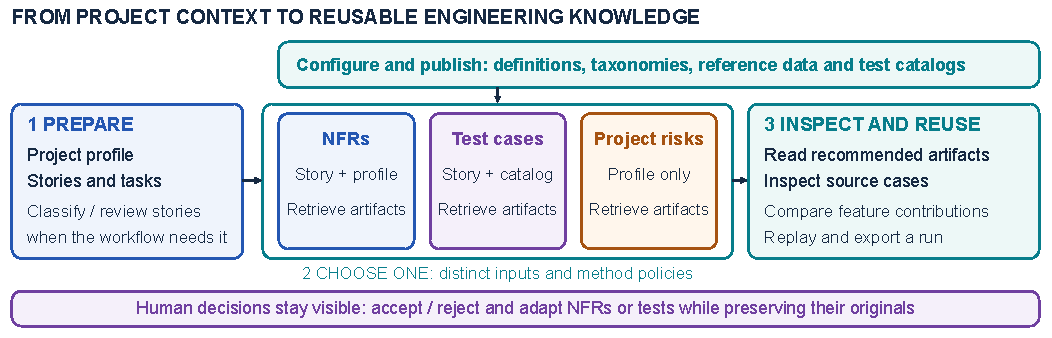
\includegraphics[width=\textwidth]{figures/recommender-workflow.pdf}

  \caption{The tool connects project preparation to three alternative recommendation workflows. Blue identifies project/story preparation, teal identifies configuration and inspection, purple identifies test reuse and human decisions, and amber identifies project risks. Labels preserve the meaning independently of color. Story classification is needed by the story-based project workflows; project risks use the profile directly.}
  \label{fig:workflow}
\end{figure*}

\subsection{Prepare once, retain project context}
In \textit{My Projects}, engineers maintain a profile, stories, and categorized tasks. Stories can be saved and edited before classification. Classification then preserves the story's identity and prepared details, so the engineer can move from preparation to recommendation without recreating the artifact.

For story-based workflows, the classification service proposes module/operation labels within the selected taxonomy. The review queue exposes model votes, rationales, and review reasons. Engineers can confirm or correct labels and record taxonomy gaps or extension proposals when the available vocabulary is insufficient. This makes uncertain classifications actionable within the workspace. Classifier confidence and agreement support routing and inspection; they are not calibrated probabilities of correctness.

\subsection{Choose the knowledge to retrieve}
The \textit{Recommenders} screen offers \textit{Non-functional requirements}, \textit{Test cases}, and \textit{Project risks}. Each choice asks for its relevant context. The story-based project workflows reuse a reviewed classification and project information; test recommendation additionally uses the fields and catalog required by its definition. Risk recommendation starts directly from the project profile.

The interface loads inputs from the selected configuration and compatible saved project values. An engineer selects a published reference dataset explicitly; the NFR workflow also offers operational history as a separate source. This makes the knowledge being consulted a visible choice. Missing values and incompatible publications are reported before the engineer proceeds.

\subsection{Inspect a suggestion before adopting it}
Results expose the recommended artifacts and the reference cases supporting them. Depending on the method, engineers can inspect selected neighbors, compared features, item contributions, and candidate exclusion reasons. For project risks, the result connects each statement to its source projects and exposes weighted feature contributions. For tests, users inspect existing test artifacts rather than generated replacements.

Figure~\ref{fig:interface} shows a preserved local result screen. The recommended statement appears alongside controls for inspecting its source, comparing features, and retaining the execution evidence.

\begin{figure*}[t]
  \centering
  % Unmodified 1425 x 2497 PNG, no DPI metadata. Graphicx clipping selects
  % the actual result area; no interface content has been redrawn.
  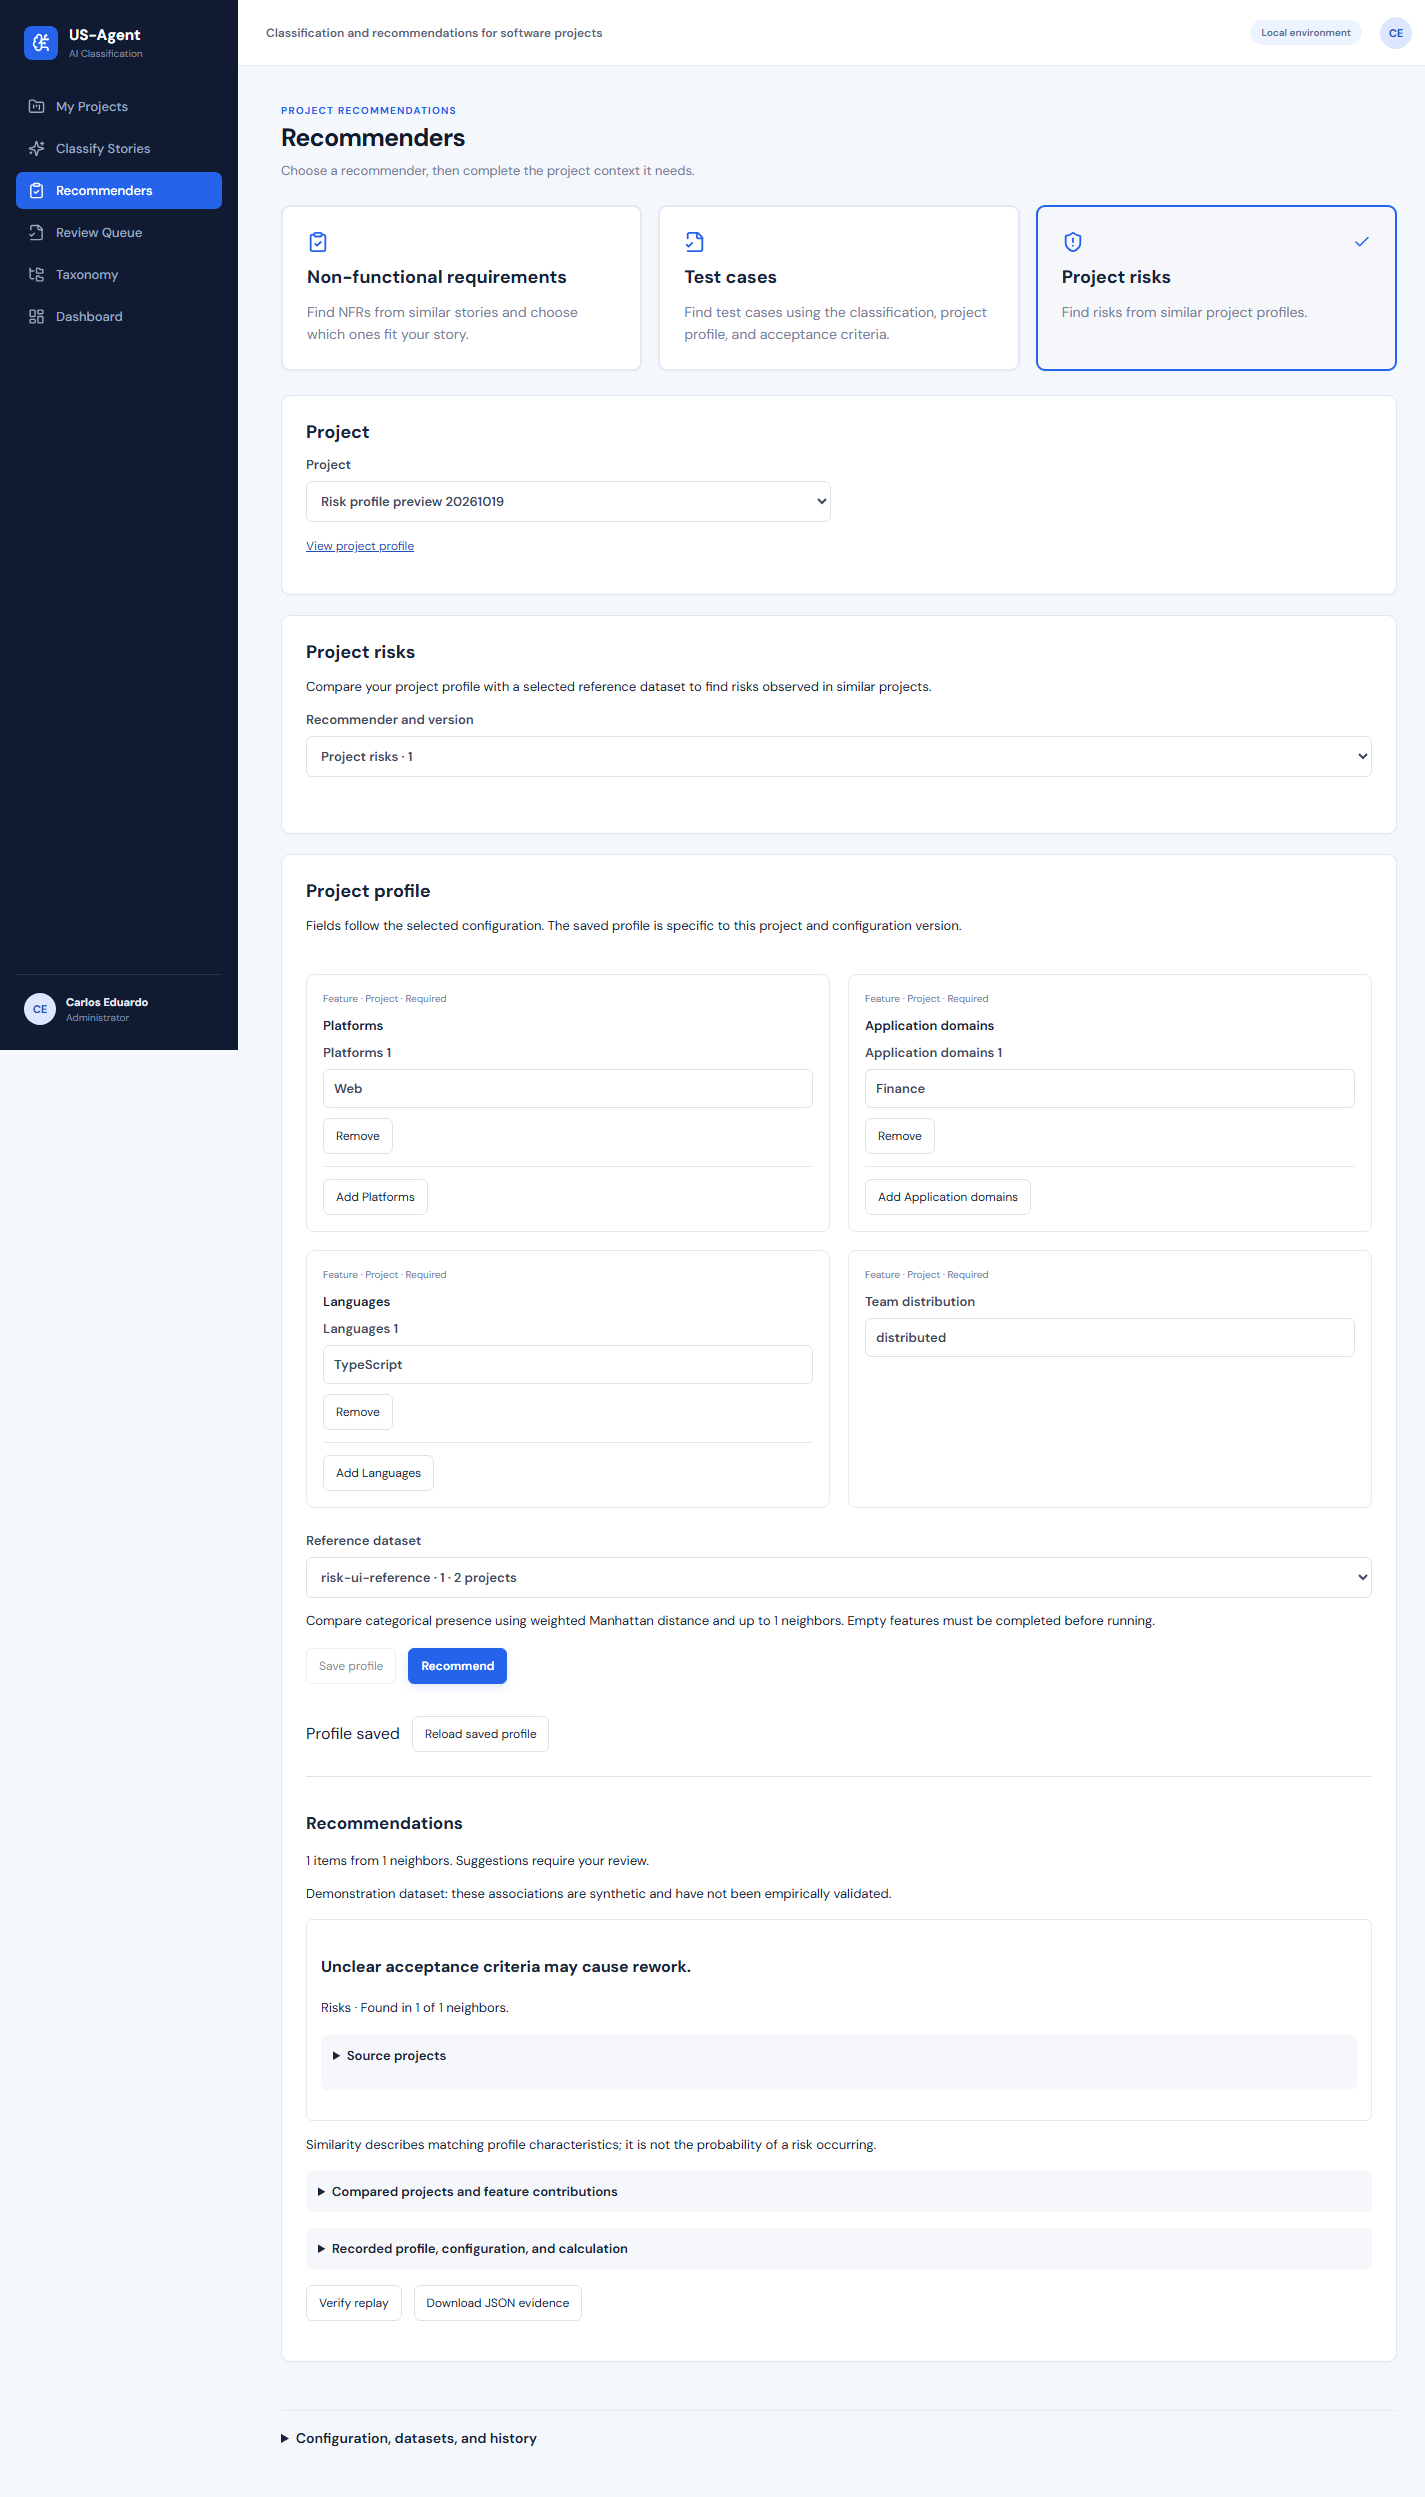
\includegraphics[width=\textwidth,trim=280bp 140bp 45bp 1775bp,clip]{figures/tool-risk-interface.png}
  \caption{Actual local-interface capture from the preserved project-risk demonstration with synthetic associations. A retrieved risk is presented with source-project inspection, compared-feature details, recorded configuration, replay, and evidence download. The viewport isolates the result area of the original capture.}
  \label{fig:interface}
\end{figure*}

NFR and test workflows support acceptance/rejection and separately versioned adaptations. An engineer can adapt an accepted NFR sentence or a test title and Gherkin steps, recording a reason while retaining the original artifact and earlier revisions. Decisions therefore enrich the reuse record without overwriting what the recommender returned. Risk suggestions currently support inspection, replay, and export; operational risk acceptance and adaptation are not implemented.

\subsection{Configure another input through the browser}
Maintainers use the configuration area to define attributes, their types and cardinalities, taxonomies, method bindings, and supported parameters. CSV/JSON import offers field mapping and a validation preview before dataset publication. Test catalogs and taxonomy lists or trees have their own publication workflows.

The distinction between a \textit{feature} and \textit{context} matters in practice: a supported categorical feature participates in calculation, while contextual metadata is validated and preserved. The project method supports adding such features and weights through configuration. Existing NFR and test policies retain their specific calculation contracts. A new field does not imply a new distance representation or a new algorithm.

\section{Demonstration: Make a Configuration Change Visible}
\label{sec:demo}
The demonstration begins with a Web/Finance/TypeScript project and declared synthetic reference cases. The presenter creates a project-risk definition, imports the supplied reference profiles, and publishes the reviewed configuration and dataset. From \textit{Recommenders}, the presenter selects the project and publications, runs the comparison, and inspects the resulting risk and source projects.

Next, the presenter creates a second definition version with a required categorical \texttt{team\_distribution} feature, weight five, and one selected neighbor. A compatible dataset version supplies the feature for each reference profile. This addition requires configuration through the interface, without a dedicated application-code field.

Figure~\ref{fig:feature} captures the resulting interaction. With the second-version definition and dataset fixed, changing only the input from \texttt{distributed} to \texttt{co-located} changes the selected source project. The presenter opens the compared features to explain the difference, then downloads each run's evidence. Similarity describes the configured profile comparison, not the probability of a risk occurring.

\begin{figure}[t]
  \centering
  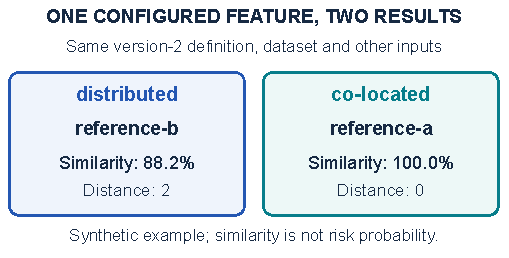
\includegraphics[width=\columnwidth]{figures/configured-feature.pdf}
  \caption{A configuration change with an observable consequence: the preserved synthetic example changes the selected neighbor when only team distribution changes. Values are read directly from the technical report.}
  \label{fig:feature}
\end{figure}

The presenter then follows the corresponding story-based route: open a prepared story, complete classification review, and request NFRs or tests. The audience can inspect an artifact's origins, record a decision, and view a separately adapted copy. This shows how the same workspace accommodates different artifact types and preserves the engineer's decisions alongside recommendation evidence.

Finally, \textit{Run history}, \textit{Verify replay}, and \textit{Download JSON evidence} expose the preserved execution. Replay compares the recorded result, explanation, and representation against a recomputation using its snapshots and compatible implementation. Earlier runs remain inspectable when the current profile or configuration changes.

\section{Implementation and Technical Evidence}
The application combines React, an Express/TypeScript API, and PostgreSQL. Definitions, taxonomies, datasets, and test catalogs are versioned publications. Executions retain their inputs, dependencies, results, explanations, and software identities. A shared nearest-neighbor kernel accepts method-specific representation, eligibility, distance, and tie-breaking policies; aggregation remains method-specific. Imported labels can be used without invoking an LLM. Organization membership assigns viewer, reviewer, maintainer, and administrator roles, with actor and audit records supporting attribution of changes.

The preserved technical package contains 23 conditions executed twice. Table~\ref{tab:conditions} retains completed, blocked, empty, and deliberately failing conditions. Eight of eight NFR compatibility outputs are preserved; all four risk conditions retain matching results, explanations, and representations. These checks establish the recorded technical behavior, rather than empirical relevance or human configuration effort. The conditions share data and are not independent samples.

\begin{table}[t]
  \caption{Technical conditions retained in the evidence package. Empty combines no candidates and no items; failed indicates deliberate technical failure.}
  \label{tab:conditions}
  \centering
  \begin{tabular}{@{}lrrrrr@{}}
    \toprule
    Example & Total & Completed & Blocked & Empty & Failed \\
    \midrule
    NFRs & 13 & 8 & 1 & 3 & 1 \\
    Tests & 6 & 3 & 1 & 1 & 1 \\
    Risks & 4 & 4 & 0 & 0 & 0 \\
    \bottomrule
  \end{tabular}
\end{table}

A proposed within-participant pilot will examine configuration, execution, inspection, replay, and export for the three tasks, recording completion, time, errors, and help requests. Methodological review and collection remain pending. Recommendation relevance and classification-error propagation require separate evaluation with independent judgments. The test and risk examples demonstrate explicit local configurations; they do not reproduce the corresponding published experiments.

\section{Related Work and Availability}
AQUSA supports user-story quality analysis~\cite{lucassen2016quality}; the reuse-oriented taxonomy links stories to development assets~\cite{dilorenzo2020wis}. Prior work also investigates LLM-based classification using that taxonomy~\cite{desouza2025automating}. These works motivate preparation and classification. NFRec, TestRec, and ARISE address recommendation of particular artifact types~\cite{ramos2025nfr,dilorenzo2026testrec,sousa2026arise}. Our demonstration centers on the implemented user journey across configuration, recommendation, source inspection, and separately recorded reuse decisions. The contribution is this configurable tool workflow and its execution evidence, rather than a new nearest-neighbor algorithm.

The demonstration materials include an operator tutorial, synthetic or reconstructed example inputs, and the preserved technical package. \draftnote{Insert verified public tool and usage-instructions URLs.} The reviewer-facing release must identify the deployed version and provide access to the demonstrated capabilities.

\section{Conclusion}
\toolname{} gives engineers a workspace for preparing project knowledge, retrieving related artifacts, understanding their origins, and preserving reuse decisions. Its three recommender configurations show how the same interaction can accommodate stories and project profiles while retaining method-specific behavior. The demonstration makes configuration tangible: a user adds a feature, observes a changed recommendation, inspects its cause, and retains the evidence.

\bibliographystyle{IEEEtran}
\bibliography{references}
\end{document}
